%%%%%%%%%%%%%%%%%%%%%%%%%%%%%%%%%%%%%%%%%%%%%%%%%%%%%%%%%%%%%%%
%% BRIEF VERSION OF OXFORD THESIS TEMPLATE FOR CHAPTER PREVIEWS

%%%%% CHOOSE PAGE LAYOUT
% format for PDF output (ie equal margins, no extra blank pages):
\documentclass[a4paper,nobind]{templates/ociamthesis}

% UL 5 January 2021 - add packages used by kableExtra
\usepackage{booktabs}
\usepackage{longtable}
\usepackage{array}
\usepackage{multirow}
\usepackage{wrapfig}
\usepackage{colortbl}
\usepackage{pdflscape}
\usepackage{tabu}
\usepackage{threeparttable}
\usepackage{threeparttablex}
\usepackage[normalem]{ulem}
\usepackage{makecell}
\usepackage[colorlinks=false,pdfpagelabels,hidelinks=]{hyperref}
\usepackage{float}


%UL set section header spacing
\usepackage{titlesec}
% 
\titlespacing\subsubsection{0pt}{24pt plus 4pt minus 2pt}{0pt plus 2pt minus 2pt}

% UL 30 Nov 2018 pandoc puts lists in 'tightlist' command when no space between bullet points in Rmd file
\providecommand{\tightlist}{%
  \setlength{\itemsep}{0pt}\setlength{\parskip}{0pt}}
 
% UL 1 Dec 2018, fix to include code in shaded environments
\usepackage{color}
\usepackage{fancyvrb}
\newcommand{\VerbBar}{|}
\newcommand{\VERB}{\Verb[commandchars=\\\{\}]}
\DefineVerbatimEnvironment{Highlighting}{Verbatim}{commandchars=\\\{\}}
% Add ',fontsize=\small' for more characters per line
\usepackage{framed}
\definecolor{shadecolor}{RGB}{248,248,248}
\newenvironment{Shaded}{\begin{snugshade}}{\end{snugshade}}
\newcommand{\AlertTok}[1]{\textcolor[rgb]{0.94,0.16,0.16}{#1}}
\newcommand{\AnnotationTok}[1]{\textcolor[rgb]{0.56,0.35,0.01}{\textbf{\textit{#1}}}}
\newcommand{\AttributeTok}[1]{\textcolor[rgb]{0.77,0.63,0.00}{#1}}
\newcommand{\BaseNTok}[1]{\textcolor[rgb]{0.00,0.00,0.81}{#1}}
\newcommand{\BuiltInTok}[1]{#1}
\newcommand{\CharTok}[1]{\textcolor[rgb]{0.31,0.60,0.02}{#1}}
\newcommand{\CommentTok}[1]{\textcolor[rgb]{0.56,0.35,0.01}{\textit{#1}}}
\newcommand{\CommentVarTok}[1]{\textcolor[rgb]{0.56,0.35,0.01}{\textbf{\textit{#1}}}}
\newcommand{\ConstantTok}[1]{\textcolor[rgb]{0.00,0.00,0.00}{#1}}
\newcommand{\ControlFlowTok}[1]{\textcolor[rgb]{0.13,0.29,0.53}{\textbf{#1}}}
\newcommand{\DataTypeTok}[1]{\textcolor[rgb]{0.13,0.29,0.53}{#1}}
\newcommand{\DecValTok}[1]{\textcolor[rgb]{0.00,0.00,0.81}{#1}}
\newcommand{\DocumentationTok}[1]{\textcolor[rgb]{0.56,0.35,0.01}{\textbf{\textit{#1}}}}
\newcommand{\ErrorTok}[1]{\textcolor[rgb]{0.64,0.00,0.00}{\textbf{#1}}}
\newcommand{\ExtensionTok}[1]{#1}
\newcommand{\FloatTok}[1]{\textcolor[rgb]{0.00,0.00,0.81}{#1}}
\newcommand{\FunctionTok}[1]{\textcolor[rgb]{0.00,0.00,0.00}{#1}}
\newcommand{\ImportTok}[1]{#1}
\newcommand{\InformationTok}[1]{\textcolor[rgb]{0.56,0.35,0.01}{\textbf{\textit{#1}}}}
\newcommand{\KeywordTok}[1]{\textcolor[rgb]{0.13,0.29,0.53}{\textbf{#1}}}
\newcommand{\NormalTok}[1]{#1}
\newcommand{\OperatorTok}[1]{\textcolor[rgb]{0.81,0.36,0.00}{\textbf{#1}}}
\newcommand{\OtherTok}[1]{\textcolor[rgb]{0.56,0.35,0.01}{#1}}
\newcommand{\PreprocessorTok}[1]{\textcolor[rgb]{0.56,0.35,0.01}{\textit{#1}}}
\newcommand{\RegionMarkerTok}[1]{#1}
\newcommand{\SpecialCharTok}[1]{\textcolor[rgb]{0.00,0.00,0.00}{#1}}
\newcommand{\SpecialStringTok}[1]{\textcolor[rgb]{0.31,0.60,0.02}{#1}}
\newcommand{\StringTok}[1]{\textcolor[rgb]{0.31,0.60,0.02}{#1}}
\newcommand{\VariableTok}[1]{\textcolor[rgb]{0.00,0.00,0.00}{#1}}
\newcommand{\VerbatimStringTok}[1]{\textcolor[rgb]{0.31,0.60,0.02}{#1}}
\newcommand{\WarningTok}[1]{\textcolor[rgb]{0.56,0.35,0.01}{\textbf{\textit{#1}}}}

%UL 2 Dec 2018 add a bit of white space before and after code blocks
\renewenvironment{Shaded}
{
  \vspace{10pt}%
  \begin{snugshade}%
}{%
  \end{snugshade}%
  \vspace{8pt}%
}
%UL 2 Dec 2018 reduce whitespace around verbatim environments
\usepackage{etoolbox}
\makeatletter
\preto{\@verbatim}{\topsep=0pt \partopsep=0pt }
\makeatother

%UL 28 Mar 2019, enable strikethrough
\usepackage[normalem]{ulem}

%UL use soul package for correction highlighting
\usepackage{soul}
\usepackage{xcolor}
\newcommand{\ctext}[3][RGB]{%
  \begingroup
  \definecolor{hlcolor}{#1}{#2}\sethlcolor{hlcolor}%
  \hl{#3}%
  \endgroup
}
\soulregister\ref7
\soulregister\cite7
\soulregister\autocite7
\soulregister\textcite7
\soulregister\pageref7

%UL 3 Nov 2019, avoid mysterious error from not having hyperref included
\usepackage{hyperref}

%%%%% SELECT YOUR DRAFT OPTIONS
% Three options going on here; use in any combination.  But remember to turn the first two off before
% generating a PDF to send to the printer!

% This adds a "DRAFT" footer to every normal page.  (The first page of each chapter is not a "normal" page.)

% This highlights (in blue) corrections marked with (for words) \mccorrect{blah} or (for whole
% paragraphs) \begin{mccorrection} . . . \end{mccorrection}.  This can be useful for sending a PDF of
% your corrected thesis to your examiners for review.  Turn it off, and the blue disappears.

%%%%% BIBLIOGRAPHY SETUP
% Note that your bibliography will require some tweaking depending on your department, preferred format, etc.
% The options included below are just very basic "sciencey" and "humanitiesey" options to get started.
% If you've not used LaTeX before, I recommend reading a little about biblatex/biber and getting started with it.
% If you're already a LaTeX pro and are used to natbib or something, modify as necessary.
% Either way, you'll have to choose and configure an appropriate bibliography format...

% The science-type option: numerical in-text citation with references in order of appearance.
% \usepackage[style=numeric-comp, sorting=none, backend=biber, doi=false, isbn=false]{biblatex}
% \newcommand*{\bibtitle}{References}

% The humanities-type option: author-year in-text citation with an alphabetical works cited.
% \usepackage[style=authoryear, sorting=nyt, backend=biber, maxcitenames=2, useprefix, doi=false, isbn=false]{biblatex}
% \newcommand*{\bibtitle}{Works Cited}

%UL 3 Dec 2018: set this from YAML in index.Rmd
\usepackage[style=numeric-comp, sorting=none, backend=biber, doi=false, isbn=false]{biblatex}
\newcommand*{\bibtitle}{References}

% This makes the bibliography left-aligned (not 'justified') and slightly smaller font.
\renewcommand*{\bibfont}{\raggedright\small}

% Change this to the name of your .bib file (usually exported from a citation manager like Zotero or EndNote).
\addbibresource{references.bib}

%%%%% YOUR OWN PERSONAL MACROS
% This is a good place to dump your own LaTeX macros as they come up.

% To make text superscripts shortcuts
	\renewcommand{\th}{\textsuperscript{th}} % ex: I won 4\th place
	\newcommand{\nd}{\textsuperscript{nd}}
	\renewcommand{\st}{\textsuperscript{st}}
	\newcommand{\rd}{\textsuperscript{rd}}

%%%%% THE ACTUAL DOCUMENT STARTS HERE
\begin{document}

%%%%% CHOOSE YOUR LINE SPACING HERE
% This is the official option.  Use it for your submission copy and library copy:
\setlength{\textbaselineskip}{22pt plus2pt}
% This is closer spacing (about 1.5-spaced) that you might prefer for your personal copies:
%\setlength{\textbaselineskip}{18pt plus2pt minus1pt}

% UL: You can set the general paragraph spacing here - I've set it to 2pt (was 0) so
% it's less claustrophobic
\setlength{\parskip}{2pt plus 1pt}

% Leave this line alone; it gets things started for the real document.
\setlength{\baselineskip}{\textbaselineskip}

% all your chapters and appendices will appear here
\hypertarget{analysis}{%
\chapter{Empirical Findings}\label{analysis}}

\minitoc 

\hypertarget{density-of-the-returns}{%
\section{Density of the returns}\label{density-of-the-returns}}

\hypertarget{mle-distribution-parameters}{%
\subsection{MLE distribution parameters}\label{mle-distribution-parameters}}

In table \ref{tab:disttable} we can see\ldots{}

\begin{verbatim}
## Warning in sqrt(diag(varcov)): NaNs produced

## Warning in sqrt(diag(varcov)): NaNs produced

## Warning in sqrt(diag(varcov)): NaNs produced
\end{verbatim}

\begin{verbatim}
## Warning in matrix(value, n, p): data length [5] is not a sub-multiple or
## multiple of the number of columns [2]
\end{verbatim}

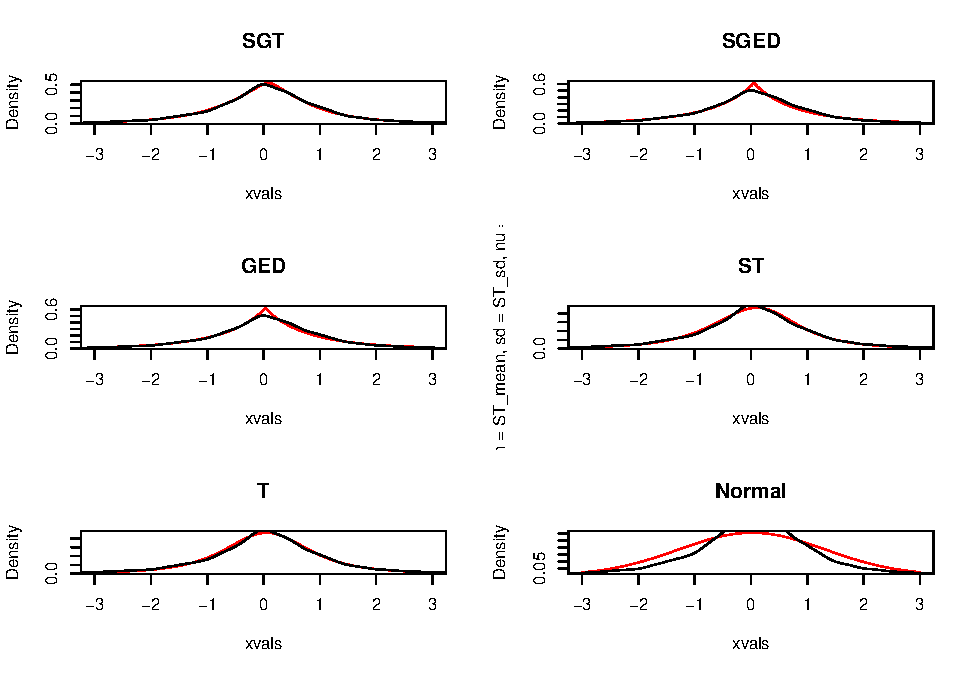
\includegraphics{04-Findings_files/figure-latex/MLE tables for diferent series-1.pdf}

\begin{table}[h!]

\caption{\label{tab:dsTable}Maximum likelihood estimates of unconditional distribution functions}
\centering
\begin{threeparttable}
\begin{tabular}[t]{lllllllrr}
\toprule
 & \$\textbackslash{}mu\$ & \$\textbackslash{}sigma\$ & \$\textbackslash{}lambda\$ & \$p\$ & \$q\$ & \$\textbackslash{}nu\$ & \$L\$ & AIC\\
\midrule
SGT & 0.02 & 1.321 & -0.04 & 1.381 & 3.317 &  & -13973.01 & 27956.01\\
 & (0.013) & (0.026) & (0.012) & (0.071) & (0.534) &  &  & \\
SGED & 0.02 & 1.274 & -0.018 & 0.918 & Inf &  & -14008.18 & 27956.01\\
 & (0.01) & (0.016) & (0.008) & (0.016) &  &  &  & \\
GED & 0.032 & 1.276 & 0 & 0.913 & Inf &  & -14009.09 & 28028.17\\
\addlinespace
 & (0.005) & (0.016) &  & (0.016) &  &  &  & \\
ST & 0.019 & 1.487 & 0.949 &  &  & 2.785 & -13997.35 & 28002.70\\
 & (0.014) & (0.056) & (0.013) &  &  & (0.1) &  & \\
T & 0.056 & 1.494 &  &  &  & 2.765 & -14005.14 & 28016.29\\
 & (0.01) & (0.056) &  &  &  & (0.097) &  & \\
\addlinespace
Normal & 0.017 & 1.304 & 0 & 2 & Inf &  & -15093.32 & 30196.64\\
 & (0.014) & (0.015) &  &  &  &  &  & \\
\bottomrule
\end{tabular}
\begin{tablenotes}
\item Notes
\end{tablenotes}
\end{threeparttable}
\end{table}

\begin{verbatim}
## Results of GARCH with constant higher moments

<!--# Here comes our main part [FILIPPO] -> to do!  -->


```r
distributions <- c("norm", "std", "sstd", "ged", "sged")
#garchspec <- garchfit <- garchforecast <- stdret <- vector(mode = "list", length = length(distributions))
#names(garchspec) <- names(garchfit) <- names(garchforecast) <- names(stdret) <- distributions
Models.garch <- c("sGARCH", "eGARCH","fGARCH.AVGARCH","fGARCH.NAGARCH", "gjrGARCH", "fGARCH.TGARCH", "iGARCH", "EWMA")

for(i in 1:length(Models.garch)){
assign(paste0("garchspec.",Models.garch[i]),vector(mode = "list", length = length(distributions)))
assign(paste0("garchfit.",Models.garch[i]),vector(mode = "list", length = length(distributions)))
assign(paste0("stdret.",Models.garch[i]),vector(mode = "list", length = length(distributions)))
} 

# ls(pattern = "garchspec.")
# sapply(ls(pattern = "garchspec."), FUN = setNames, distributions)

#.sGARCH--------------------------
for(i in 1:length(distributions)){
# Specify a GARCH model with constant mean
garchspec.sGARCH[[i]] <- ugarchspec(mean.model = list(armaOrder = c(1,0)),
                     variance.model = list(model = "sGARCH", garchOrder = c(1,1), variance.targeting = F), 
                     distribution.model = distributions[i])
# Estimate the model
garchfit.sGARCH[[i]] <- ugarchfit(data = R, spec = garchspec.sGARCH[[i]])
# Compute stdret using residuals()
stdret.sGARCH[[i]] <- residuals(garchfit.sGARCH[[i]], standardize = TRUE)
}

#.eGARCH-------------------
for(i in 1:length(distributions)){
# Specify a GARCH model with constant mean
garchspec.eGARCH[[i]] <- ugarchspec(mean.model = list(armaOrder = c(1,0)),
                     variance.model = list(model = "eGARCH", variance.targeting = F), 
                     distribution.model = distributions[i])
# Estimate the model
garchfit.eGARCH[[i]] <- ugarchfit(data = R, spec = garchspec.eGARCH[[i]])
# Compute stdret using residuals()
stdret.eGARCH[[i]] <- residuals(garchfit.eGARCH[[i]], standardize = TRUE)
}

#.fGARCH.NAGARCH------------------------
for(i in 1:length(distributions)){
# Specify a GARCH model with constant mean
garchspec.fGARCH.NAGARCH[[i]] <- ugarchspec(mean.model = list(armaOrder = c(1,0)),
                     variance.model = list(model = "fGARCH", submodel = "NAGARCH", variance.targeting = F),
                     distribution.model = distributions[i])
# Estimate the model
garchfit.fGARCH.NAGARCH[[i]] <- ugarchfit(data = R, spec = garchspec.fGARCH.NAGARCH[[i]])
# Compute stdret using residuals()
stdret.fGARCH.NAGARCH[[i]] <- residuals(garchfit.fGARCH.NAGARCH[[i]], standardize = TRUE)
}

#.fGARCH.AVGARCH------------------------
for(i in 1:length(distributions)){
# Specify a GARCH model with constant mean
garchspec.fGARCH.AVGARCH[[i]] <- ugarchspec(mean.model = list(armaOrder = c(1,0)),
                     variance.model = list(model = "fGARCH", submodel = "AVGARCH", variance.targeting = F),
                     distribution.model = distributions[i])
# Estimate the model
garchfit.fGARCH.AVGARCH[[i]] <- ugarchfit(data = R, spec = garchspec.fGARCH.AVGARCH[[i]])
# Compute stdret using residuals()
stdret.fGARCH.AVGARCH[[i]] <- residuals(garchfit.fGARCH.AVGARCH[[i]], standardize = TRUE)
}

#.gjrGARCH------------------
for(i in 1:length(distributions)){
# Specify a GARCH model with constant mean
garchspec.gjrGARCH[[i]] <- ugarchspec(mean.model = list(armaOrder = c(1,0)),
                     variance.model = list(model = "gjrGARCH", variance.targeting = F), 
                     distribution.model = distributions[i])
# Estimate the model
garchfit.gjrGARCH[[i]] <- ugarchfit(data = R, spec = garchspec.gjrGARCH[[i]])
# Compute stdret using residuals()
stdret.gjrGARCH[[i]] <- residuals(garchfit.gjrGARCH[[i]], standardize = TRUE)
}

#fGARCH.TGARCH-------------------
for(i in 1:length(distributions)){
# Specify a GARCH model with constant mean
garchspec.fGARCH.TGARCH[[i]] <- ugarchspec(mean.model = list(armaOrder = c(1,0)),
                     variance.model = list(model = "fGARCH", submodel = "TGARCH", variance.targeting = F), 
                     distribution.model = distributions[i])
# Estimate the model
garchfit.fGARCH.TGARCH[[i]] <- ugarchfit(data = R, spec = garchspec.fGARCH.TGARCH[[i]])
# Compute stdret using residuals()
stdret.fGARCH.TGARCH[[i]] <- residuals(garchfit.fGARCH.TGARCH[[i]], standardize = TRUE)
}

#.iGARCH--------------------
for(i in 1:length(distributions)){
# Specify a GARCH model with constant mean
garchspec.iGARCH[[i]] <- ugarchspec(mean.model = list(armaOrder = c(1,0)),
                     variance.model = list(model = "iGARCH", variance.targeting = F), 
                     distribution.model = distributions[i])
# Estimate the model
garchfit.iGARCH[[i]] <- ugarchfit(data = R, spec = garchspec.iGARCH[[i]])
# Compute stdret using residuals()
stdret.iGARCH[[i]] <- residuals(garchfit.iGARCH[[i]], standardize = TRUE)
}

#.csGARCH-----------------
# for(i in 1:length(distributions)){
# # Specify a GARCH model with constant mean
# garchspec.csGARCH[[i]] <- ugarchspec(mean.model = list(armaOrder = c(1,0)),
#                      variance.model = list(model = "csGARCH", variance.targeting = F),
#                      distribution.model = distributions[i])
# # Estimate the model
# garchfit.csGARCH[[i]] <- ugarchfit(data = R, spec = garchspec.csGARCH[[i]])
# # Compute stdret using residuals()
# stdret.csGARCH[[i]] <- residuals(garchfit.csGARCH[[i]], standardize = TRUE)
# }


# we need EWMA
for(i in 1:length(distributions)){
# Specify a GARCH model with constant mean
garchspec.EWMA[[i]] <- ugarchspec(mean.model = list(armaOrder = c(1,0)),
                     variance.model = list(model = "iGARCH", variance.targeting = F),
                     distribution.model = distributions[i], fixed.pars = list(omega=0))
# Estimate the model
garchfit.EWMA[[i]] <- ugarchfit(data = R, spec = garchspec.EWMA[[i]])
# Compute stdret using residuals()
stdret.EWMA[[i]] <- residuals(garchfit.EWMA[[i]], standardize = TRUE)
}


#  make the histogram
# 
# chart.Histogram(stdret.iGARCH[[1]], methods = c("add.normal","add.density" ),
#                 colorset = c("gray","red","blue"))
\end{verbatim}

\begin{Shaded}
\begin{Highlighting}[]
\NormalTok{table3 }\OtherTok{\textless{}{-}} \FunctionTok{matrix}\NormalTok{(}\AttributeTok{nrow =} \DecValTok{12}\NormalTok{, }\AttributeTok{ncol =} \DecValTok{5}\NormalTok{)}
\FunctionTok{colnames}\NormalTok{(table3) }\OtherTok{\textless{}{-}}\NormalTok{ distributions}

\CommentTok{\#trying a loop, maybe you can solve that @filippo?}
\DocumentationTok{\#\# column loop i = normal distribution, std, sstd, ged, sged}
\NormalTok{table3[}\DecValTok{1}\NormalTok{,}\DecValTok{1}\NormalTok{] }\OtherTok{\textless{}{-}}\NormalTok{ garchfit.sGARCH[[}\DecValTok{1}\NormalTok{]]}\SpecialCharTok{@}\NormalTok{fit}\SpecialCharTok{$}\NormalTok{coef[}\DecValTok{1}\NormalTok{] }\CommentTok{\#first parameter estimate}
\NormalTok{table3[}\DecValTok{2}\NormalTok{,}\DecValTok{1}\NormalTok{] }\OtherTok{\textless{}{-}}\NormalTok{ garchfit.sGARCH[[}\DecValTok{1}\NormalTok{]]}\SpecialCharTok{@}\NormalTok{fit}\SpecialCharTok{$}\NormalTok{se.coef[}\DecValTok{1}\NormalTok{] }\CommentTok{\#first standard error}
\NormalTok{table3[}\DecValTok{3}\NormalTok{,}\DecValTok{1}\NormalTok{] }\OtherTok{\textless{}{-}}\NormalTok{ garchfit.sGARCH[[}\DecValTok{1}\NormalTok{]]}\SpecialCharTok{@}\NormalTok{fit}\SpecialCharTok{$}\NormalTok{coef[}\DecValTok{2}\NormalTok{] }\CommentTok{\#second parameter estimate}
\NormalTok{table3[}\DecValTok{4}\NormalTok{,}\DecValTok{1}\NormalTok{] }\OtherTok{\textless{}{-}}\NormalTok{ garchfit.sGARCH[[}\DecValTok{1}\NormalTok{]]}\SpecialCharTok{@}\NormalTok{fit}\SpecialCharTok{$}\NormalTok{se.coef[}\DecValTok{2}\NormalTok{]}



\CommentTok{\#...}
\NormalTok{table3 }\OtherTok{\textless{}{-}} \FunctionTok{round}\NormalTok{(table3, }\DecValTok{3}\NormalTok{)}

\CommentTok{\# for (i in length(distributions)) \{}
\CommentTok{\#   for (j in nrow(table3)) \{}
\CommentTok{\#     table3[j,i] \textless{}{-} garchfit.sGARCH[[i]]@fit$coef}
\CommentTok{\#     table3[j+1,i] \textless{}{-}garchfit.sGARCH[[i]]@fit$se.coef}
\CommentTok{\#     \}}
\CommentTok{\# \}}

\FunctionTok{print}\NormalTok{(}\StringTok{"sGARCH"}\NormalTok{)}
\NormalTok{garchfit.sGARCH[[}\DecValTok{1}\NormalTok{]]}\SpecialCharTok{@}\NormalTok{fit}\SpecialCharTok{$}\NormalTok{coef}
\NormalTok{garchfit.sGARCH[[}\DecValTok{1}\NormalTok{]]}\SpecialCharTok{@}\NormalTok{fit}\SpecialCharTok{$}\NormalTok{se.coef}
\end{Highlighting}
\end{Shaded}

\begin{Shaded}
\begin{Highlighting}[]
\FunctionTok{print}\NormalTok{(}\StringTok{"iGARCH"}\NormalTok{)}
\NormalTok{garchfit.iGARCH[[}\DecValTok{1}\NormalTok{]]}\SpecialCharTok{@}\NormalTok{fit}\SpecialCharTok{$}\NormalTok{coef}
\NormalTok{garchfit.iGARCH[[}\DecValTok{1}\NormalTok{]]}\SpecialCharTok{@}\NormalTok{fit}\SpecialCharTok{$}\NormalTok{se.coef}
\end{Highlighting}
\end{Shaded}

\begin{Shaded}
\begin{Highlighting}[]
\FunctionTok{print}\NormalTok{(}\StringTok{"EWMA"}\NormalTok{)}
\NormalTok{garchfit.EWMA[[}\DecValTok{1}\NormalTok{]]}\SpecialCharTok{@}\NormalTok{fit}\SpecialCharTok{$}\NormalTok{coef}
\FunctionTok{c}\NormalTok{(garchfit.EWMA[[}\DecValTok{1}\NormalTok{]]}\SpecialCharTok{@}\NormalTok{fit}\SpecialCharTok{$}\NormalTok{se.coef[}\DecValTok{1}\SpecialCharTok{:}\DecValTok{2}\NormalTok{],}\ConstantTok{NA}\NormalTok{,garchfit.EWMA[[}\DecValTok{1}\NormalTok{]]}\SpecialCharTok{@}\NormalTok{fit}\SpecialCharTok{$}\NormalTok{se.coef[}\DecValTok{3}\NormalTok{], }\ConstantTok{NA}\NormalTok{)}
\end{Highlighting}
\end{Shaded}

\begin{Shaded}
\begin{Highlighting}[]
\FunctionTok{print}\NormalTok{(}\StringTok{"eGARCH"}\NormalTok{)}
\NormalTok{garchfit.eGARCH[[}\DecValTok{1}\NormalTok{]]}\SpecialCharTok{@}\NormalTok{fit}\SpecialCharTok{$}\NormalTok{coef}
\NormalTok{garchfit.eGARCH[[}\DecValTok{1}\NormalTok{]]}\SpecialCharTok{@}\NormalTok{fit}\SpecialCharTok{$}\NormalTok{se.coef}
\end{Highlighting}
\end{Shaded}

\begin{Shaded}
\begin{Highlighting}[]
\FunctionTok{print}\NormalTok{(}\StringTok{"gjrGARCH"}\NormalTok{)}
\NormalTok{garchfit.gjrGARCH[[}\DecValTok{1}\NormalTok{]]}\SpecialCharTok{@}\NormalTok{fit}\SpecialCharTok{$}\NormalTok{coef}
\NormalTok{garchfit.gjrGARCH[[}\DecValTok{1}\NormalTok{]]}\SpecialCharTok{@}\NormalTok{fit}\SpecialCharTok{$}\NormalTok{se.coef}
\end{Highlighting}
\end{Shaded}

\begin{Shaded}
\begin{Highlighting}[]
\FunctionTok{print}\NormalTok{(}\StringTok{"NAGARCH"}\NormalTok{)}
\NormalTok{garchfit.fGARCH.NAGARCH[[}\DecValTok{1}\NormalTok{]]}\SpecialCharTok{@}\NormalTok{fit}\SpecialCharTok{$}\NormalTok{coef}
\NormalTok{garchfit.fGARCH.NAGARCH[[}\DecValTok{1}\NormalTok{]]}\SpecialCharTok{@}\NormalTok{fit}\SpecialCharTok{$}\NormalTok{se.coef}
\end{Highlighting}
\end{Shaded}

\begin{Shaded}
\begin{Highlighting}[]
\FunctionTok{print}\NormalTok{(}\StringTok{"TGARCH"}\NormalTok{)}
\NormalTok{garchfit.fGARCH.TGARCH[[}\DecValTok{1}\NormalTok{]]}\SpecialCharTok{@}\NormalTok{fit}\SpecialCharTok{$}\NormalTok{coef}
\NormalTok{garchfit.fGARCH.TGARCH[[}\DecValTok{1}\NormalTok{]]}\SpecialCharTok{@}\NormalTok{fit}\SpecialCharTok{$}\NormalTok{se.coef}
\end{Highlighting}
\end{Shaded}

\begin{Shaded}
\begin{Highlighting}[]
\FunctionTok{print}\NormalTok{(}\StringTok{"TSGARCH/AVGARCH"}\NormalTok{)}
\NormalTok{garchfit.fGARCH.AVGARCH[[}\DecValTok{1}\NormalTok{]]}\SpecialCharTok{@}\NormalTok{fit}\SpecialCharTok{$}\NormalTok{coef}
\NormalTok{garchfit.fGARCH.AVGARCH[[}\DecValTok{1}\NormalTok{]]}\SpecialCharTok{@}\NormalTok{fit}\SpecialCharTok{$}\NormalTok{se.coef}
\end{Highlighting}
\end{Shaded}

\hypertarget{results-of-garch-with-time-varying-higher-moments}{%
\section{Results of GARCH with time-varying higher moments}\label{results-of-garch-with-time-varying-higher-moments}}

\begin{Shaded}
\begin{Highlighting}[]
\FunctionTok{require}\NormalTok{(racd)}
\FunctionTok{require}\NormalTok{(rugarch)}
\FunctionTok{require}\NormalTok{(parallel)}
\FunctionTok{require}\NormalTok{(xts)}
\CommentTok{\# ACD specification}
\NormalTok{sGARCH\_ACDspec }\OtherTok{=} \FunctionTok{acdspec}\NormalTok{(}\AttributeTok{mean.model =} \FunctionTok{list}\NormalTok{(}\AttributeTok{armaOrder =} \FunctionTok{c}\NormalTok{(}\DecValTok{1}\NormalTok{, }\DecValTok{0}\NormalTok{)), }\AttributeTok{variance.model =} \FunctionTok{list}\NormalTok{(}\AttributeTok{variance.targeting =} \ConstantTok{TRUE}\NormalTok{),}
\AttributeTok{distribution.model =} \FunctionTok{list}\NormalTok{(}\AttributeTok{model =} \StringTok{\textquotesingle{}jsu\textquotesingle{}}\NormalTok{, }\AttributeTok{skewOrder =} \FunctionTok{c}\NormalTok{(}\DecValTok{1}\NormalTok{, }\DecValTok{1}\NormalTok{, }\DecValTok{1}\NormalTok{), }\AttributeTok{shapeOrder =} \FunctionTok{c}\NormalTok{(}\DecValTok{1}\NormalTok{,}\DecValTok{1}\NormalTok{,}\DecValTok{1}\NormalTok{), }\AttributeTok{skewmodel =} \StringTok{\textquotesingle{}quad\textquotesingle{}}\NormalTok{, }\AttributeTok{shapemodel =} \StringTok{\textquotesingle{}pwl\textquotesingle{}}\NormalTok{))}

\CommentTok{\# sGARCH}
\NormalTok{cl }\OtherTok{=} \FunctionTok{makePSOCKcluster}\NormalTok{(}\DecValTok{10}\NormalTok{)}
\NormalTok{fit }\OtherTok{=} \FunctionTok{acdfit}\NormalTok{(sGARCH\_ACDspec, }\FunctionTok{as.data.frame}\NormalTok{(R), }\AttributeTok{solver =} \StringTok{\textquotesingle{}msoptim\textquotesingle{}}\NormalTok{, }\AttributeTok{solver.control =} \FunctionTok{list}\NormalTok{(}\AttributeTok{restarts =} \DecValTok{10}\NormalTok{),}\AttributeTok{cluster =}\NormalTok{ cl) }\CommentTok{\#very long process: starts from different starting values to find an optimum}
\end{Highlighting}
\end{Shaded}

\begin{Shaded}
\begin{Highlighting}[]
\CommentTok{\# plotxts comes from implementing https://stackoverflow.com/a/50051183/271616}
\CommentTok{\# par(mfrow = c(2, 2), mai = c(0.75, 0.75, 0.3, 0.3))}
\CommentTok{\# cm \textless{}{-} plot.zoo(xts(fit@model$modeldata$data, fit@model$modeldata$index), auto.grid = FALSE,minor.ticks = FALSE, main = \textquotesingle{}Conditional Mean\textquotesingle{},yaxis.right = F, col = \textquotesingle{}steelblue\textquotesingle{})}
\CommentTok{\# cm \textless{}{-} lines(fitted(fit), col = 2)}
\CommentTok{\# cm}
\CommentTok{\# cs \textless{}{-} plot(xts(abs(fit@model$modeldata$data),fit@model$modeldata$index), auto.grid = FALSE,}
\CommentTok{\# minor.ticks = FALSE, main = \textquotesingle{}Conditional Sigma\textquotesingle{}, yaxis.right = F,col = \textquotesingle{}grey\textquotesingle{})}
\CommentTok{\# cs \textless{}{-} lines(sigma(fit), col = \textquotesingle{}steelblue\textquotesingle{})}
\CommentTok{\# cs}
\CommentTok{\# plot(racd::skewness(fit), col = \textquotesingle{}steelblue\textquotesingle{},yaxis.right = F, main = \textquotesingle{}Conditional Skewness\textquotesingle{})}
\CommentTok{\# plot(racd::kurtosis(fit), col = \textquotesingle{}steelblue\textquotesingle{}, yaxis.right = F,main = \textquotesingle{}Conditional Excess Kurtosis\textquotesingle{})}

\CommentTok{\# pnl \textless{}{-} function(fitted(fit),xts(fit@model$modeldata$data, fit@model$modeldata$index), ...) \{}
\CommentTok{\#   panel.number \textless{}{-} parent.frame()$panel.number}
\CommentTok{\#   if (panel.number == 1) lines(fitted(fit), xts(fit@model$modeldata$data, fit@model$modeldata$index),col = "red")}
\CommentTok{\#   lines(fitted(fit),xts(fit@model$modeldata$data, fit@model$modeldata$index), col = "red")}
\CommentTok{\# \}}
\CommentTok{\# plot(xts(fit@model$modeldata$data, fit@model$modeldata$index), auto.grid = T,minor.ticks = FALSE,major.ticks=T, yaxis.right = F, main = \textquotesingle{}Conditional Mean\textquotesingle{}, col = \textquotesingle{}steelblue\textquotesingle{}, xlab = "", screens = 1, ylab="") \#panel = pnl}
\CommentTok{\# \# lines(fitted(fit), col = 2) + grid()}
\CommentTok{\# }
\CommentTok{\# plot(xts(fit@model$modeldata$data, fit@model$modeldata$index), auto.grid = T,minor.ticks = FALSE,major.ticks=T, yaxis.right = F, main = \textquotesingle{}Conditional Mean\textquotesingle{}, col = \textquotesingle{}steelblue\textquotesingle{}, xlab = "", screens = 1, ylab="", )}
\end{Highlighting}
\end{Shaded}



%%%%% REFERENCES

% JEM: Quote for the top of references (just like a chapter quote if you're using them).  Comment to skip.
% \begin{savequote}[8cm]
% The first kind of intellectual and artistic personality belongs to the hedgehogs, the second to the foxes \dots
%   \qauthor{--- Sir Isaiah Berlin \cite{berlin_hedgehog_2013}}
% \end{savequote}

\setlength{\baselineskip}{0pt} % JEM: Single-space References

{\renewcommand*\MakeUppercase[1]{#1}%
\printbibliography[heading=bibintoc,title={\bibtitle}]}

\end{document}
